%%%%%%%%%%%%%%%%%%%%%%%%%%%%%%%%%%%%%%%%%%%%%%%%%%%%%%%%%%%%%%%%%%%%%%%%
%%%%%%%%%%%%%%%%%%%%%% Simple LaTeX CV Template %%%%%%%%%%%%%%%%%%%%%%%%
%%%%%%%%%%%%%%%%%%%%%%%%%%%%%%%%%%%%%%%%%%%%%%%%%%%%%%%%%%%%%%%%%%%%%%%%

%%%%%%%%%%%%%%%%%%%%%%%%%%%%%%%%%%%%%%%%%%%%%%%%%%%%%%%%%%%%%%%%%%%%%%%%
%% NOTE: If you find that it says                                     %%
%%                                                                    %%
%%                           1 of ??                                  %%
%%                                                                    %%
%% at the bottom of your first page, this means that the AUX file     %%
%% was not available when you ran LaTeX on this source. Simply RERUN  %%
%% LaTeX to get the ``??'' replaced with the number of the last page  %%
%% of the document. The AUX file will be generated on the first run   %%
%% of LaTeX and used on the second run to fill in all of the          %%
%% references.                                                        %%
%%%%%%%%%%%%%%%%%%%%%%%%%%%%%%%%%%%%%%%%%%%%%%%%%%%%%%%%%%%%%%%%%%%%%%%%

%%%%%%%%%%%%%%%%%%%%%%%%%%%% Document Setup %%%%%%%%%%%%%%%%%%%%%%%%%%%%


% Don't like 10pt? Try 11pt or 12pt
\documentclass[10pt,a4paper]{article}
\RequirePackage[T1]{fontenc}

% The automated optical recognition software used to digitize resume
% information works best with fonts that do not have serifs. This
% command uses a sans serif font throughout. Uncomment both lines (or at
% least the second) to restore a Roman font (i.e., a font with serifs).
\usepackage{times}
\renewcommand{\familydefault}{\sfdefault}

% The OCR software also has a hard time with italics. These commands get
% rid of the two common ways to italicize text in LaTeX. Get rid of them
% to turn italics back on.
\renewcommand\emph[1]{#1}
\renewcommand\textit[1]{\underline{#1}}

% This is a helpful package that puts math inside length specifications
\usepackage{calc}

% This package helps LaTeX auto-hyphenate hyphenated words if you use
% special hyphens. For example, bio\-/mimicry will properly hyphenate
% ``mimicry'' if necessary.
\usepackage[shortcuts]{extdash}

% Layout: Puts the section titles on left side of page
\reversemarginpar

%
%         PAPER SIZE, PAGE NUMBER, AND DOCUMENT LAYOUT NOTES:
%
% The next \usepackage line changes the layout for CV style section
% headings as marginal notes. It also sets up the paper size as either
% letter or A4. By default, letter was used. If A4 paper is desired,
% comment out the letterpaper lines and uncomment the a4paper lines.
%
% As you can see, the margin widths and section title widths can be
% easily adjusted.
%
% ALSO: Notice that the includefoot option can be commented OUT in order
% to put the PAGE NUMBER *IN* the bottom margin. This will make the
% effective text area larger.
%
% IF YOU WISH TO REMOVE THE ``of LASTPAGE'' next to each page number,
% see the note about the +LP and -LP lines below. Comment out the +LP
% and uncomment the -LP.
%
% IF YOU WISH TO REMOVE PAGE NUMBERS, be sure that the includefoot line
% is uncommented and ALSO uncomment the \pagestyle{empty} a few lines
% below.
%

%% Use these lines for letter-sized paper
% \usepackage[paper=letterpaper,
%             %includefoot, % Uncomment to put page number above margin
%             marginparwidth=1.2in,     % Length of section titles
%             marginparsep=.05in,       % Space between titles and text
%             margin=1in,               % 1 inch margins
%             includemp]{geometry}

%% Use these lines for A4-sized paper
\usepackage[paper=a4paper,
           %includefoot, % Uncomment to put page number above margin
           marginparwidth=30.5mm,    % Length of section titles
           marginparsep=1.5mm,       % Space between titles and text
           margin=25mm,              % 25mm margins
           includemp]{geometry}

%% More layout: Get rid of indenting throughout entire document
\setlength{\parindent}{0in}

% Provides special list environments and macros to create new ones
\usepackage[shortlabels]{enumitem}

% Simpler bibsections for CV sections
% (thanks to natbib for inspiration)
%
% * For lists of references with hanging indents and no numbers:
%
%   \begin{bibsection}
%       \item ...
%   \end{bibsection}
%
% * For numbered lists of references (with hanging indents):
%
%   \begin{bibenum}
%       \item ...
%   \end{bibenum}
%
%   Note that bibenum numbers continuously throughout. To reset the
%   counter, use
%
%   \restartlist{bibenum}
%
%   at the place where you want the numbering to reset.
\usepackage{graphicx,wrapfig}



\makeatletter
\newlength{\bibhang}
\setlength{\bibhang}{1em}
\newlength{\bibsep}
 {\@listi \global\bibsep\itemsep \global\advance\bibsep by\parsep}
\newlist{bibsection}{itemize}{3}
\setlist[bibsection]{label=,leftmargin=\bibhang,%
        itemindent=-\bibhang,
        itemsep=\bibsep,parsep=\z@,partopsep=0pt,
        topsep=0pt}
\newlist{bibenum}{enumerate}{3}
\setlist[bibenum]{label=[\arabic*],resume,leftmargin={\bibhang+\widthof{[999]}},%
        itemindent=-\bibhang,
        itemsep=\bibsep,parsep=\z@,partopsep=0pt,
        topsep=0pt}
\let\oldendbibenum\endbibenum
\def\endbibenum{\oldendbibenum\vspace{-.6\baselineskip}}
\let\oldendbibsection\endbibsection
\def\endbibsection{\oldendbibsection\vspace{-.6\baselineskip}}
\makeatother

%%% Setup header and footer (with page number and possible last page)
%
% The first block sets up pages 2--end
% The second block sets up page 1 formatting
%
%%%
%
% NOTE: comment the +LP lines and uncomment the -LP lines to have page
%       numbers without the ``of ##'' last page reference)
%
% NOTE: uncomment the \pagestyle{empty} line to get rid of all page
%       numbers on pages 2--end. To get rid of page numbers on page 1,
%       comment out the \thispagestyle{plain} line on the first page
%       below.
%       (also make sure includefoot is commented out above)
%
\usepackage{fancyhdr,lastpage}
\pagestyle{fancy}
%\pagestyle{empty}      % Uncomment this to get rid of page numbers
\fancyhf{}\renewcommand{\headrulewidth}{0pt}
\fancyfootoffset{\marginparsep+\marginparwidth}
\newlength{\footpageshift}
\setlength{\footpageshift}
          {0.5\textwidth+0.5\marginparsep+0.5\marginparwidth-2in}

%%%% PAGES 2--9 NUMBERING:
%% These two lines put page number in upper-right corner of pages 2--end
\rhead{Richard, p.~\arabic{page} of \protect\pageref*{LastPage}}   % +LP
%\rhead{Pavlic, p.~\arabic{page}}                                 % -LP

%% These lines put page number in bottom (center) of pages 2--end
%\lfoot{\hspace{\footpageshift}%
%       \parbox{4in}{\, \hfill %
%                    \arabic{page} of \protect\pageref*{LastPage} % +LP
%%                    \arabic{page}                               % -LP
%                    \hfill \,}}
%%%% END PAGE 2--9 NUMBERING

%%%% PAGE 1 NUMBERING:
\makeatletter
\let\oldps@plain\ps@plain
\renewcommand{\ps@plain}{\oldps@plain%
\renewcommand{\@evenfoot}{\hspace*{-\footpageshift}\hfil %
   Richard, p.~\arabic{page} of \protect\pageref*{LastPage} % +LP
%    p.~\arabic{page}                               % -LP
    \hfil}%
\renewcommand{\@oddfoot}{\@evenfoot}}
\makeatother
%%%% END PAGE 1 NUMBERING

% Finally, give us PDF bookmarks and colored links
%
% NOTE: Some OCR software might be negatively affected by hyperlinks. So
%       most employers recommend the draft option here. Alternatively,
%       making all links black (as opposed to darkblue) should hopefully
%       prevent problems with most OCR.
%
% (to enable hyperlinks and bookmarks, comment out ``draft'' line;
%  to disable hyperlinks and bookmarks, uncomment ``draft'' line)
\usepackage{color,hyperref}
%\definecolor{darkblue}{rgb}{0.0,0.0,0.3}
\hypersetup{breaklinks,colorlinks,
            linkcolor=blue,urlcolor=blue,
            anchorcolor=blue,citecolor=blue,pdfstartview={XYZ null null 1.00}
            %linkcolor=darkblue,urlcolor=darkblue,
            %anchorcolor=darkblue,citecolor=darkblue,
            %draft
            }
\usepackage{marvosym} % for telephone
%%%%%%%%%%%%%%%%%%%%%%%% End Document Setup %%%%%%%%%%%%%%%%%%%%%%%%%%%%


%%%%%%%%%%%%%%%%%%%%%%%%%%% Helper Commands %%%%%%%%%%%%%%%%%%%%%%%%%%%%

%%% HEADING AT TOP OF CURRICULUM VITAE

% The title (name) with a horizontal rule under it
% (optional argument typesets an object right-justified across from name
%  as well)
%
% Usage: \makeheading{name}
%        OR
%        \makeheading[right_object]{name}
%
% Place at top of document. It should be the first thing.
% If ``right_object'' is provided in the square-braced optional
% argument, it will be right justified on the same line as ``name'' at
% the top of the CV. For example:
%
%       \makeheading[\emph{Curriculum vitae}]{Your Name}
%
% will put an emphasized ``Curriculum vitae'' at the top of the document
% as a title. Likewise, a picture could be included:
%
%   \makeheading[{\includegraphics[height=1.5in]{my_picture}}]{Your Name}
%
% the picture will be flush right across from the name. For this example
% to work, make sure the extra set of curly braces is included. Also
% makes ure that \usepackage{graphicx} is somewhere in the preamble.
\newcommand{\makeheading}[2][]%
        {\hspace*{-\marginparsep minus \marginparwidth}%
         \begin{minipage}[t]{\textwidth+\marginparwidth+\marginparsep}%
             {\large \bfseries #2 \hfill #1}\\[-0.15\baselineskip]%
                 \rule{\columnwidth}{1pt}%
         \end{minipage}}

%%% SECTION HEADINGS

% The section headings. Flush left in small caps down pseudo-margin.
%
% Usage: \section{section name}
\renewcommand{\section}[1]{\pagebreak[3]%
    \vspace{1.3\baselineskip}%
    \phantomsection\addcontentsline{toc}{section}{#1}%
    \noindent\llap{\scshape\smash{\parbox[t]{\marginparwidth}{\hyphenpenalty=10000\raggedright #1}}}%
    \vspace{-\baselineskip}\par}

%%% LISTS

% This macro alters a list by removing some of the space that follows the list
% (is used by lists below)
\newcommand*\fixendlist[1]{%
    \expandafter\let\csname preFixEndListend#1\expandafter\endcsname\csname end#1\endcsname
    \expandafter\def\csname end#1\endcsname{\csname preFixEndListend#1\endcsname\vspace{-0.6\baselineskip}}}

% These macros help ensure that items in outer-type lists do not get
% separated from the next line by a page break
% (they are used by lists below)
\let\originalItem\item
\newcommand*\fixouterlist[1]{%
    \expandafter\let\csname preFixOuterList#1\expandafter\endcsname\csname #1\endcsname
    \expandafter\def\csname #1\endcsname{\csname preFixOuterList#1\endcsname\let\oldItem\item\def\item{\pagebreak[2]\oldItem}}
    \expandafter\let\csname preFixOuterListend#1\expandafter\endcsname\csname end#1\endcsname
    \expandafter\def\csname end#1\endcsname{\let\item\oldItem\csname preFixOuterListend#1\endcsname}}
\newcommand*\fixinnerlist[1]{%
    \expandafter\let\csname preFixInnerList#1\expandafter\endcsname\csname #1\endcsname
    \expandafter\def\csname #1\endcsname{\let\oldItem\item\let\item\originalItem\csname preFixInnerList#1\endcsname}
    \expandafter\let\csname preFixInnerListend#1\expandafter\endcsname\csname end#1\endcsname
    \expandafter\def\csname end#1\endcsname{\csname preFixInnerListend#1\endcsname\let\item\oldItem}}

% An itemize-style list with lots of space between items
%
% Usage:
%   \begin{outerlist}
%       \item ...    % (or \item[] for no bullet)
%   \end{outerlist}
\newlist{outerlist}{itemize}{3}
    \setlist[outerlist]{label=\enskip\textbullet,leftmargin=*}
    \fixendlist{outerlist}
    \fixouterlist{outerlist}

% An environment IDENTICAL to outerlist that has better pre-list spacing
% when used as the first thing in a \section
%
% Usage:
%   \begin{lonelist}
%       \item ...    % (or \item[] for no bullet)
%   \end{lonelist}
\newlist{lonelist}{itemize}{3}
    \setlist[lonelist]{label=\enskip\textbullet,leftmargin=*,partopsep=0pt,topsep=0pt}
    \fixendlist{lonelist}
    \fixouterlist{lonelist}

% An itemize-style list with little space between items
%
% Usage:
%   \begin{innerlist}
%       \item ...    % (or \item[] for no bullet)
%   \end{innerlist}
\newlist{innerlist}{itemize}{3}
    \setlist[innerlist]{label=\enskip\textbullet,leftmargin=*,parsep=0pt,itemsep=0pt,topsep=0pt,partopsep=0pt}
    \fixinnerlist{innerlist}

% An environment IDENTICAL to innerlist that has better pre-list spacing
% when used as the first thing in a \section
%
% Usage:
%   \begin{loneinnerlist}
%       \item ...    % (or \item[] for no bullet)
%   \end{loneinnerlist}
\newlist{loneinnerlist}{itemize}{3}
    \setlist[loneinnerlist]{label=\enskip\textbullet,leftmargin=*,parsep=0pt,itemsep=0pt,topsep=0pt,partopsep=0pt}
    \fixendlist{loneinnerlist}
    \fixinnerlist{loneinnerlist}

%%% EXTRA SPACE

% To add some paragraph space between lines.
% This also tells LaTeX to preferably break a page on one of these gaps
% if there is a needed pagebreak nearby.
\newcommand{\blankline}{\quad\pagebreak[3]}
\newcommand{\halfblankline}{\quad\vspace{-0.5\baselineskip}\pagebreak[3]}

%%% FORMATTING MACROS

% Provides a linked \doi{#1} that links doi:#1 to http://dx.doi.org/#1
\usepackage{doi}
% To change the text before the DOI, adjust this command
%\renewcommand\doitext{doi:}

% Provides a linked \url{#1} that doesn't require escape characters
\usepackage{url}

% You can adjust the style \url{} uses here:
% (options are: same, rm, sf, tt; defaults to tt)
\urlstyle{same}

% For \email{ADDRESS}, links ADDRESS to the url mailto:ADDRESS
% (uncomment to typeset the e\-/mail address in typewriter font;
%  otherwise, will be typeset in the \urlstyle above)
%\DeclareUrlCommand\emaillink{\urlstyle{tt}}
\providecommand*\emaillink[1]{\nolinkurl{#1}}
\providecommand*\email[1]{\href{mailto:#1}{\emaillink{#1}}}

\providecommand\BibTeX{{B\kern-.05em{\sc i\kern-.025em b}\kern-.08em \TeX}}
\providecommand\Matlab{\textsc{Matlab}}

% Custom hyphenation rules for words that LaTeX has trouble with
\hyphenation{bio-mim-ic-ry bio-in-spi-ra-tion re-us-a-ble pro-vid-er Media-Wiki}

%%%%%%%%%%%%%%%%%%%%%%%% End Helper Commands %%%%%%%%%%%%%%%%%%%%%%%%%%%

%%%%%%%%%%%%%%%%%%%%%%%%% Begin CV Document %%%%%%%%%%%%%%%%%%%%%%%%%%%%

\begin{document}
\thispagestyle{plain}
    

\makeheading[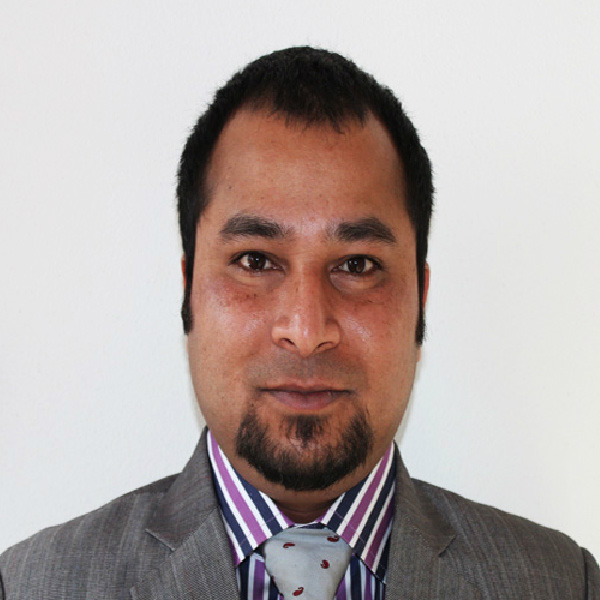
\includegraphics{richard11}]{Curriculum Vitae}


%\section{Contact Information}

\section{Personal Information}

% NOTE: Mind where the & separators and \\ breaks are in the following
%       table. Table is one row made up of three parboxes. The left
%       parbox has address info, the middle parbox has a vertical bar,
%       and the right parbox has phone and electronic contact
%       information.
%
% MACROS: \rcollength is the width of the right column of the table
%             (adjust it to your liking; default is 1.85in).
%         \spacewidth is width of area between left and right boxes.
%
\newlength{\rcollength}\setlength{\rcollength}{1.85in}%
\newlength{\spacewidth}\setlength{\spacewidth}{20pt}
%
\begin{tabular}[t]{@{}p{\textwidth-\rcollength-\spacewidth}@{}p{\spacewidth}@{}p{\rcollength}}%

% Address box
\parbox{\textwidth-\rcollength-\spacewidth}{%
% \Letter~Via Della Resistenza 64, Int H, Povo,\\
%     Trento - 38123, Italy. \\
Full Name: \textbf{Supta Richard Philip}\\
Date of Birth: July 6th, 1983\\
Place of Birth: Gazipur, Bangladesh\\
Marital Status: Married \\
Gender: Male

}

&
% Uncomment to add a vertical bar in middle of contact information
%{\vrule width 0.5pt}
\parbox[m][5\baselineskip]{\spacewidth}{} &

% Non-snail-mail contact information
\parbox{\rcollength}{%
Albjergparken 1, 6 D\o r 4,\\
2660, Br\o ndby Strand,\\
	Denmark.
\Telefon~+45 42325773 \\
   %\Mundus~\url{www.supta.info} \\
  \Email~\href{mailto:supta.philip@gmail.com}{supta.philip@gmail.com} \\
  %\MartinVogel ~\href{https://github.com/suptaphilip}{github.com/suptaphilip}\\
   \raisebox{-1pt}{
\includegraphics[height=9pt]{github.pdf}}~\href{https://github.com/suptaphilip}{github.com/suptaphilip}\\
  %\Mundus~\href{https://github.com/suptaphilip}{github.com/suptaphilip}
}

\end{tabular}

%%
%% In modern CV's, it seems like ``Objective'' is frowned upon. Instead,
%% incorporate it into a well-constructed cover letter. The ``More
%% information'' can go at the end of the CV, but it should not distract
%% from the section giving references available to contact.
%%
%

\section{Personal Profile}
A Computer Science Graduate with strong analytical, technical and
research skills in Human Computer Interaction (HCI), software engineering, interaction design, artificial intelligence, Data Management and Analysis; have graduated from university of Trento, Italy. Now I am seeking a research position related to my interest.
% \section{Objective}
%
% Full-time position that allows for advanced research in electrical and
% computer engineering (communications, control, software, electronics,
% and sustainability), with a particular focus on complex distributed
% systems (i.e., modeling, analysis, design, and verification)
% \begin{innerlist}
%     \item For more information, see \url{http://www.tedpavlic.com/engjobsearch/}
% \end{innerlist}

% \section{Qualifications and Interests}
% 
% Software Engineering, Requirements Engineering, Human Computer Interaction, User
% Study \& Evaluation, Programming in Java, php and python, Ontology and Domain
% Development, Data Analysis, Machine Learning.

% \section{Availability}
% 
% \begin{loneinnerlist}
%     \item Start time is negotiable; may be possible to start immediately
%     \item Geographic location is flexible, but there is preference
%         for Tempe, AZ
% \end{loneinnerlist}
% 
% \section{Security Clearance}
% 
% Department of Defense Top Secret SCI with polygraph (expired: 2002)
% 
% % \section{Citizenship}
% %
% % USA


\section{Education}

\href{http://www.unitn.it/en}{\textbf{University of Trento}},
Trento, Italy.
\begin{outerlist}
\item[] M.Sc.,
        \href{http://disi.unitn.it/}
             {Computer Science}, July 2013
             \hfill Result:  90 (out of 110)
        \begin{innerlist}
        \item Thesis Title: \emph{``Smart Cafeteria'' Adaptive And Interactive Mobile Application}
        \item Adviser:
              \href{http://disi.unitn.it/~deangeli/homepage/doku.php?id=home}
                   {Professor Antonella De Angeli}
        \item Area of Study: Software Technologies
        \item Resources: \url{http://suptaphilip.github.io/Master-Thesis/}
        \end{innerlist}
\end{outerlist}
\ \\
\href{http://www.aiub.edu/}{\textbf{American International University-Bangladesh}},
Dhaka, Bangladesh.
\begin{outerlist}
\item[] B.Sc.,
        \href{http://www.aiub.edu/}
             {Computer Science \& Engineering}, January 2008
             \hfill GPA: 3.78 (4.0 scale)
        \begin{innerlist}
        \item Thesis Title: \emph{Autonomous Robot Navigation Using Optical Mouse-based Odometry, Line Following and End Of Line Detection.}
        \item Adviser: Professor Shakil Mahbubul Huq
        \item Resources: \url{https://github.com/suptaphilip/Bachelor-Thesis}
        \end{innerlist}
\end{outerlist}

\section{Professional Experience}

\href{www.hesburger.fi}{\textbf{Hesburger Ltd.}},
Dhaka, Bangladesh.
\begin{outerlist}

    \item[] \textit{Program Designer}%
            \hfill \textbf{March 22, 2009 to August 17, 2010}
            \begin{innerlist}
                \item Supervisor:
                        \href{http://fi.linkedin.com/pub/tuomas-karkkainen/4a/586/113}%
                           {Tuomas karkkainen}\\
					 \Email~Email : \href{mailto:tuomas.karkkainen@gurulogic.fi}{tuomas.karkkainen@gurulogic.fi}\\
    				\Mundus~\url{www.hesburger.fi}
                \item Analysis applications requirements, design database,
                writing technical documents, coding, fixing bugs and worked as LAMP full stack developer(PHP).
               
            \end{innerlist}

\end{outerlist}

\halfblankline

\href{www.bengalsols.com}{\textbf{Bengal Solutions Ltd.}},
Dhaka, Bangladesh.
\begin{outerlist}

    \item[] \textit{Software Engineer}%
            \hfill \textbf{August 1, 2007 to March 20, 2009}
            \begin{innerlist}
                \item Supervisor:
                        \href{http://bd.linkedin.com/in/mkafi}%
                             {Abdul Al Kafi}\\
					 \Email~Email : \href{mailto:kafi@bengalsols.com }{kafi@bengalsols.com}\\
    				\Mundus~\url{www.bengalsols.com}
                \item Analysis Web Application requirements, design database,
                prepare technical documents, writing code in PHP
                Frameworks(CakePHP, CodeIgniter) and testing the application and
                fixing bugs.
               
            \end{innerlist}

\end{outerlist}

%\halfblankline

%\vspace{0.1in}

\section{Publications}

\begin{bibenum}
    \item Autonomous Robot Navigation system And Line Following Robot.\\
    \emph{LAP LAMBERT Academic Publishing (May 7, 2012)\\
	Authors: Supta Richard Philip, Amlan Chowdhury, Tohedul Islam.\\
	ISBN-13: 978-3659108556}.\\
	 \url{http://www.amazon.com/dp/3659108553}

    
\end{bibenum}

% Add a little space to nudge next ``Conference Publications'' marginpar
% down to make room for tall ``Submitted Conference Publications''
% marginpar. If there are enough submitted journal publications, this
% space will not be needed (and should be removed).
%\vspace{0.1in}



\section{Course Projects at Masters}
The following projects/reports have been done in Masters
%
\begin{innerlist}
\item Computer Security : POPS/ Java Card Case Study - Software Update Scenario.
\item Human Computer Interaction : The Use Of Collaborative Software in a
Learning context by designing a standard wiki.
\item Concurrency Theory : Knuths Algorithm Mutual Exclusion using CCS in
Concurrency Workbench.
\item Requirement Engineering : Online Apparel Buying House Management System.
\item Network Security : Secure SMS in Android.
%\item Logics for Data and Knowledge Management: Domain and Ontology development
%using protege.
\end{innerlist}
%\halfblankline


\section{Professional Development}
I was involved in the following projects in my job
\begin{innerlist}
\item Hesburger Databank \url{http://databank.hesburger.fi} [Cake PHP and MySQL]
\item Gurulogic Systems \url{http://www.gurulogic.com.bd/} [PHP and MySQL]
\item Banchte Shekha \url{http://banchteshekha.org} [PHP and MySQL]
\item MCCHSL \url{http://mcchsl.org/} [Codeigniter and MySQL]
\end{innerlist}

%\halfblankline


% \section{Courses in Masters}
% \begin{loneinnerlist}
%  \item \emph{Human Computer Interaction:} Usability analysis, Pact analysis, Evaluation
% and Prototype designing.
% \item \emph{Formal Methods:} Linear Temporal Logic(LTL), Computational Tree
% Logic(CTL), CTL Model Checking, LTL Model Checking,Bounded Model Checking, Time
% Automata.This course was introduced about SPIN, NuSMV tools.
%     
% \item \emph{Mathematical Logic:} Propositional Logic, ClassL, First Order Logic,
% Modal Logic.This course was introduced about logic and domain, their semantics.
%        
% \item \emph{Logics for Data and Knowledge Management:}  Description Logic, Modal
% Logic, Context Logic, RDF, OWL, RelBAC(Description Logic, Terminology Box and
% Assumption Box using Description Logic.
%     
% \item  \emph{Agent-oriented Software Engineering:} Multi-agent system, Deductive
% reasoning, BDI, Goal analysis, Agent oriented methodologies, Tropos, JADE.
% 
% \item \emph{Computability:} Set theory, induction,Programming languages \&
% computational power, Lambda calculus, Enumeration of programs, Logical
% characterization of recursive functions: primitive and general recursion, Problem
% classes: decidable and semi-decidable,Church's Thesis,Kleene's theorem, Rice's
% fixed point theorem, Rice-Shapiro theorem,m-Reductions
% 	
% \item \emph{Computational complexity:} Complexity Classes P, NP and
% NP-Completeness, The search problem, The decision problem, Time Complexity, Space
% Complexity, Time versus Space, Polynomial-time Reductions, Logarithmic Space
% , PSPACE, Probabilistic Polynomial-Time,Probabilistic Proof Systems, Interactive
% Proof Systems, Zero-Knowledge Proof Systems.
% 	
% \item \emph{Concurrency theory:} Petri Nets; CCS; Operational and bisimulation
% semantics; basics of domain theory; Modal and temporal logics.
% 		
% \item \emph{Programming languages: semantics:}  Introduction of Syntax and semantics,
% Operational, denotational and axiomatic semantics, Static and dynamic semantics,
% Transition systems, Structural Operational Semantics, Imperative languages-
% expressions, statements, declarations, procedure; Functional languages-
% expressions and functions
% 
% \item \emph{Requirement Engineering:} Goal analysis, Feasibility study, Goal
% modeling, Business Rules, Object Constraint Language (OCL), UML diagrams,
% Requirements Specifications.
%     
% \item \emph{Network Security:} practical encryption and deception techniques,
% firewalls , SNORT;
%       
% \item \emph{ Computer Security:} defining potential threats, defining actors and their
% goals,  RBAC.
% \end{loneinnerlist}

\section{Academic Awards}
% \begin{innerlist}
% \item 
Full Academic Scholarships for Masters of Science which includes the full
waiver of the tuition fees and covers living expenses for full 2.5 years.\\
Awarded by:\href{http://www.operauni.tn.it/}{Opera Universitaria di Trento}, Provincia Autonoma di Trento, Italy.
\href{http://www.unitn.it/en}{University of Trento.}
%\end{innerlist}


\section{Technical Skill And Expertise}

\textbf{Operating systems:} Mac, Linux Ubuntu, Windows.

% \halfblankline
% \begin{innerlist}
% \item Linux Ubuntu, Windows.
% \end{innerlist}

% \halfblankline

\textbf{Programming Languages:} Java, C, PHP, HTML, CSS, Java Script, Beginner in Python, Ruby, C\# and node.js.

% \halfblankline
% 
% \begin{innerlist}
% \item Java, PHP, HTML, CSS, Java Script, C, C++, UML 2.0,
% Latex.
% \item Beginner in Python, Ruby and Matlab scripting.
% \end{innerlist}
% 
% \halfblankline

\textbf{Databases:} MySQL, SQLite, Oracle Express Edition.

% \halfblankline
% 
% \begin{innerlist}
% \item MySQL, SQLite, Oracle Express Edition.
% \end{innerlist}
% 
% \halfblankline


\textbf{Frameworks:} MVC, Cake PHP, CodeIgniter.

% \halfblankline
% 
% \begin{innerlist}
% \item MVC, Cake PHP, CodeIgniter.
% \end{innerlist}
% 
% \halfblankline


\textbf{Technologies:} JSP, Servlet, JAXB, Web Service REST,Twitter Bootstrap, Android.

\textbf{Software quality assurance (SQA):} Have knowledge about SQA methods; Unit Testing, Black Box Testing, White Box Testing and Usability testing.


\textbf{Eclipse IDE:} Having a good knowledge about Eclipse IDE in java
development (jsp, servlet, JDBC, Hibernate), Eclipse CDT (C and C++ in MinGW
GCC), PyDev plug-in for Eclipse (Python 2.6).


\textbf{Latex:} Scientific Report writing, Articles writing with the IEEE
      Transactions format using Latex, Presentation Beamer using Latex.
      Bibliography Referencing style apa, ieeetr, acm.


\textbf{LAMP:} Having a good knowledge in Linux, Apache HTTP
Server, MySQL and PHP Bundle.

\textbf{SVN:} Having a sound knowledge in svn and git.
%


\section{Interests}

Collecting E-Book about Technologies and Courses, Google searching and
reading article and blogs, Watching Football, Cricket, documentary and tutorials
in youtube.

% \halfblankline
% 
% \begin{innerlist}
% \item JSP, Servlet, JAXB, Web Service REST,Twitter Bootstrap, Android.
% \end{innerlist}
% 
% \halfblankline


% \section{Expertise}
% 
% \textbf{Eclipse IDE:} Having a good knowledge about Eclipse IDE in java
% development (jsp, servlet, JDBC, Hibernate), Eclipse CDT (C and C++ in MinGW
% GCC), PyDev plug-in for Eclipse (Python 2.6).

% \begin{innerlist}
% \item Expert in Eclipse : Having a good knowledge about Eclipse IDE in java
% development (jsp, servlet, JDBC, Hibernate), Eclipse CDT (C and C++ in MinGW
% GCC), PyDev plug-in for Eclipse (Python 2.6).
% \end{innerlist}
% 
% \halfblankline

% \textbf{Latex:} Scientific Report writing, Articles writing with the IEEE
%       Transactions format using Latex, Presentation Beamer using Latex.
%       Bibliography Referencing style apa, ieeetr, acm.
%
% \begin{innerlist}
% \item Latex (Expert in MiKTeX + TeXnicCenter and MiKTeX
%       +TeXlipse): Scientific Report writing, Articles writing with the IEEE
%       Transactions format using Latex, Presentation Beamer using Latex.\\
% Bibliography Referencing style with Latex : apa, ieeetr, acm.
% 
% \end{innerlist}
% 
% \halfblankline

%\textbf{LAMP:} Having a good knowledge in Linux, Apache HTTP
%Server, MySQL and PHP Bundle.
%
% \begin{innerlist}
%  \item Expert in LAMP: Having a good knowledge in Linux, Apache HTTP
% Server, MySQL and PHP Bundle.
% 
% \end{innerlist}
% 
% \halfblankline

%\textbf{SVN:} Having a sound knowledge in svn and git.
%
% \begin{innerlist}
%    \item Expert in SVN: Having a sound knowledge in svn and git.
% 
% \end{innerlist}
% 
% \halfblankline

%\textbf{Prototyping tools:} Having a good knowledge in Balsamiq.
%
% \begin{innerlist}
%    \item Expert in Prototyping tools : Having a good knowledge in Balsamiq
% Mockups.
% 
% \end{innerlist}
% 
% \halfblankline

% \textbf{Graphics and Diagram:}
% %
% \begin{innerlist}
%     \item Expert in Graphics and diagram : Having a good knowledge in Dia
% Diagram Editor for UML and many conceptual diagram;GLE(Graphics Layout Engine) for
% graphics scripting language designed for creating publication quality graphs,
% plots, diagrams and figures.
% \end{innerlist}


% \section{Public Profile}
% \begin{outerlist}
% \item \textbf{Linkedin}: \url{http://www.linkedin.com/in/richardphilip}\\
% \item \textbf{GitHub}: \url{https://github.com/suptaphilip}\\
% %\item \textbf{Blog}: \url{http://richardsphilip.wordpress.com}
% %\item \textbf{Blog}: \url{http://supta.info/}
%   \end{outerlist}
% \vspace{0.1in}


%\section{Language skills}



% Add a little space to nudge next ``More Information'' marginpar
% down to make room for tall ``References Available to Contact''
% marginpar.
%\vspace{0.1in}
\section{References}
%Available upon request. \\ \\
	{\bfseries Antonella De Angeli} \\
	Associate Professor of Human-Computer Interaction,\\
	Department of Information Engineering and Computer Science,\\
	University of Trento, Italy.\\
	\Telefon~: +39-0461-882052 -- Fax: +39-0461-882093 \\
	\Letter~: \href{mailto:antonella.deangeli@disi.unitn.it}{antonella.deangeli@disi.unitn.it}\\
   \Mundus~: \url{http://disi.unitn.it/~deangeli/homepage/doku.php}\\
   
 %   	{\bfseries Khandaker Tabin Hasan} \\
	% Assistant Professor,\\
	% American International University - Bangladesh.\\
	% \Letter~: \href{mailto: tabin@aiub.edu}{ tabin@aiub.edu}\\
	% \Mundus~: \url{http://www.aiub.edu/} \\	
	% Courtesy Professor, KnowDive Research Group,\\
	% University of Trento.\\
	% \Letter~: \href{mailto:tabin@disi.unitn.it}{tabin@disi.unitn.it}\\
	%  \Mundus~: \url{http://disi.unitn.it/~knowdive/Members.php} \\ \\	

	
	% {\bfseries Tuomas K\"{a}rkk\"{a}inen} \\
	% CTO at Gurulogic Microsystems\\
	% \Letter~: \href{mailto:tuomas.karkkainen@gurulogic.fi}{tuomas.karkkainen@gurulogic.fi}\\
 %    \Mundus~: \url{http://gurulogic.com/} \\ \\	

\vspace{-8pt} \rule{\textwidth}{1pt}

\begin{center}
  \begin{small}
    Last Updated: \today
  \end{small}
\end{center}

\end{document}

%%%%%%%%%%%%%%%%%%%%%%%%%% End CV Document %%%%%%%%%%%%%%%%%%%%%%%%%%%%%

%----------------------------------------------------------------------%
% The following is copyright and licensing information for
% redistribution of this LaTeX source code; it also includes a liability
% statement. If this source code is not being redistributed to others,
% it may be omitted. It has no effect on the function of the above code.
%----------------------------------------------------------------------%
% Copyright (c) 2007, 2008, 2009, 2010, 2011 by Theodore P. Pavlic
%
% Unless otherwise expressly stated, this work is licensed under the
% Creative Commons Attribution-Noncommercial 3.0 United States License. To
% view a copy of this license, visit
% http://creativecommons.org/licenses/by-nc/3.0/us/ or send a letter to
% Creative Commons, 171 Second Street, Suite 300, San Francisco,
% California, 94105, USA.
%
% THE SOFTWARE IS PROVIDED "AS IS", WITHOUT WARRANTY OF ANY KIND, EXPRESS
% OR IMPLIED, INCLUDING BUT NOT LIMITED TO THE WARRANTIES OF
% MERCHANTABILITY, FITNESS FOR A PARTICULAR PURPOSE AND NONINFRINGEMENT.
% IN NO EVENT SHALL THE AUTHORS OR COPYRIGHT HOLDERS BE LIABLE FOR ANY
% CLAIM, DAMAGES OR OTHER LIABILITY, WHETHER IN AN ACTION OF CONTRACT,
% TORT OR OTHERWISE, ARISING FROM, OUT OF OR IN CONNECTION WITH THE
% SOFTWARE OR THE USE OR OTHER DEALINGS IN THE SOFTWARE.
%----------------------------------------------------------------------%